%/!\ ici on parle en terme d'architecture, donc ce qu'on a décidé AVANT d'implémenter


\section{L'architecture générale}

Nous avons choisi dès le départ de suivre une architecture de type MVC, et nous nous y sommes tenu tout au long du projet. Afin de nous facilité le découpage du code, et de définir nos principales interfaces nous
avons conçu au démarrage du projet une architecture globale. Elle est représentée dans la figure \ref{Architecture}. %METTRE l'image Archi.png

\begin{figure}[h!]
\centering
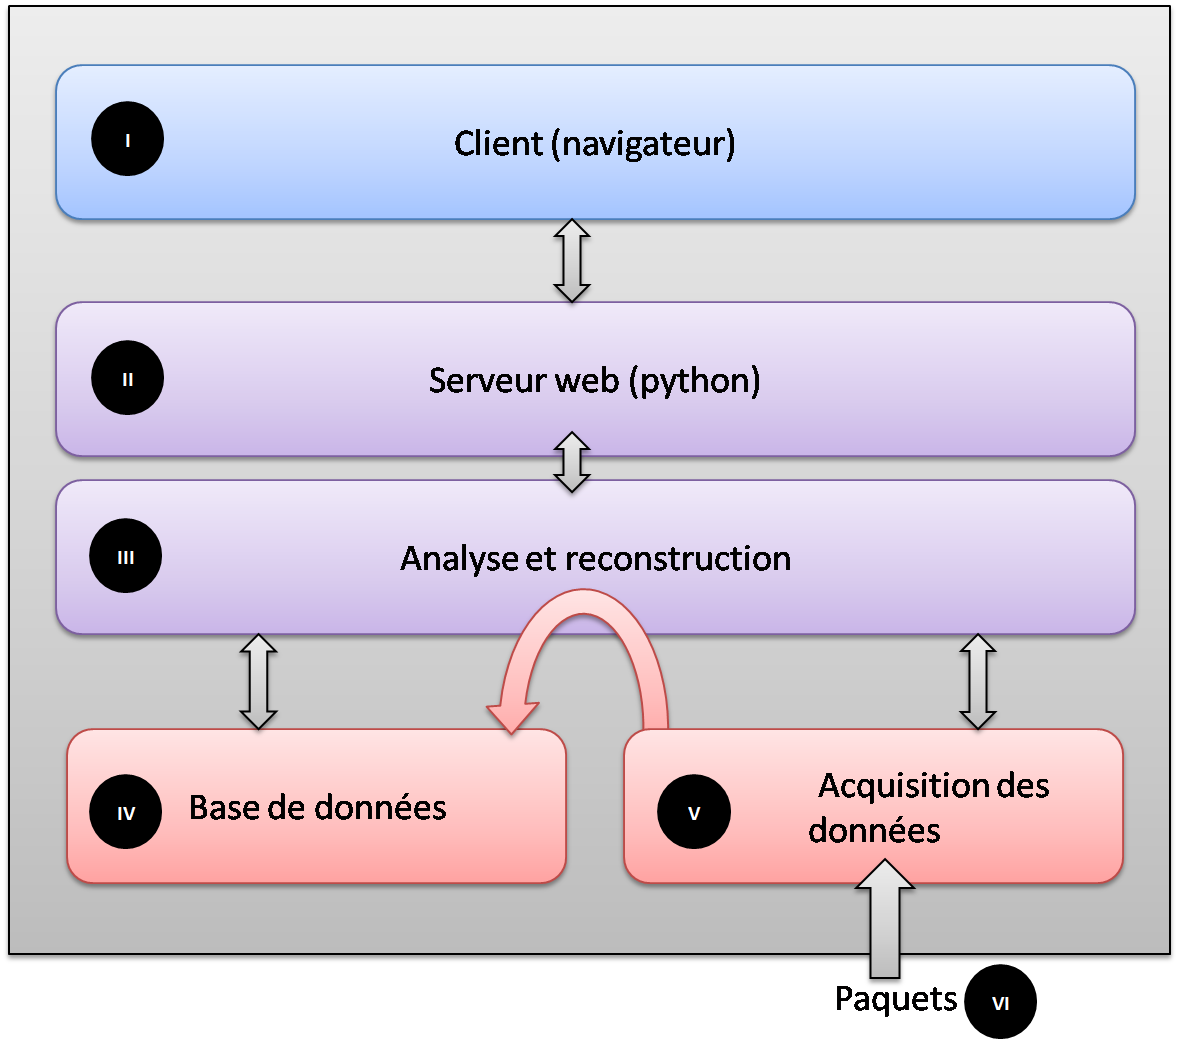
\includegraphics[scale=0.5]{Archi.png}
\caption{Architecture de Sniffeirb}
\label{Architecture}
\end{figure}

Nous avons choisi d'utiliser le langage python pour notre projet, en parti pour ses nombreuses bibliothèques, y compris pour les captures réseaux. De plus nous avions tous envi d'approfondir nos connaissances dans 
un langage de programmation autre que le C,C++ ou java.

\section{Excplication du rôle des différentes couches}

\subsection{Client}
Le client est soit le terminal dans lequel on lance le programme, soit un navigateur web. Nous n'offrons pas tout à fait les même service sur ces deux interfaces, ceci est lié à notre volonté d'avoir une interface utilisateur simple. 
De ce fait, le terminal permet seulement de lancer une capture, ou de lancer le programme avec différentes options (lancement du serveur web, choix d'une ancienne capture à charger, choix du nom de la nouvelle capture..).
L'interface web permet de lancer une capture, d'afficher les flux des différentes communications, de reconstruire les documents et de changer certain paramètres.

Le navigateur utilise des requêtes ajax afin d'interagir avec  le programme.
Dans le but de fournir un programme utilisable sur le plus grand nombre de navigateur possible, nous avons utilisé des frameworks reconnus dans le milieu. Nous avons donc choisi d'utiliser JQuery pour nos requêtes, Bootstrap pour la mise en page et le css, et DataTables pour la présentation des flux sous forme de tableau. 

\subsection{Serveur web}
Le serveur web est l'interface entre les requêtes html provenant du client, et vers les différentes actions possibles du sniffer. Après avoir lancé une action le serveur renvoie si besoin est des données au client au format
JSON.
Nous avons choisi d'utiliser JSON pour plusieurs raisons. C'est un format de données structuré, moins verbeux que le xml, et qui est très bien intégré avec le javascript et le python. 

\subsection{Analyse et reconstruction}
Ce composant analyse une communication pour determiner son protocole, reconstruit les flux possibles et reconstruit les documents qui transitent en donnant un pourcentage de validité. Nous n'assurons seulement la reconstruction des documents sur le protocle html pour le moment (page html et images).

\subsection{Base de données}
La base de données sert à stocker les paquets réseau regroupé par communication.	Stocker les données nous permet de rejouer des échanges de données (soit pour le débugage, soit suite à une amélioration algorithmique du projet).	
Nous avons choisi d'utiliser une base no-sql mongo pour ses performances et sa souplesse. Elle s'utilise aisément en python grâce au module pymongo.

\subsection{Acquisition des données}
Ce composant récupère les données réseau, et les met dans la base de données. Les paquets sont regroupé par communications.
Nous utilisons le module scapy de python afin de récupérer les paquets. Il est de plus au niveau que la lib pcap ou winpcacp, ce qui facilite la capture des paquêts réseau.

\subsection{Paquets}
Ceci représente le réseau, et les paquets qui circulent. En paramétrant la carte réseau

\section{La base du sniffer : la récupération des paquets et leur stockage}


\section{La reconstruction...}

\subsection{... des flux}

\subsection{... puis des documents}

\section{L'affichage}

\section{Choix des outils}
-python
-javascript

